\documentclass{article}

\usepackage{geometry}

\usepackage{amsmath}
\usepackage{amsthm}
\usepackage{amssymb}

%\usepackage{authblk}
\usepackage{graphicx}
\usepackage[backend=biber]{biblatex}
\addbibresource{references.bib}
\usepackage{enumerate}
\usepackage{caption}
\usepackage{subcaption}
%\usepackage{float}

\usepackage[colorlinks]{hyperref}
\usepackage{cleveref}

%\usepackage{multicol}
% \usepackage{listings} % for code blocks

\theoremstyle{definition}
\newtheorem{theorem}{Theorem}[section]
\newtheorem{lemma}[theorem]{Lemma}
\newtheorem{proposition}[theorem]{Proposition}
\newtheorem{definition}[theorem]{Definition}
\newtheorem{conjecture}[theorem]{Conjecture}
\newtheorem{remark}[theorem]{Remark}
\numberwithin{equation}{section}

\title{Periodic traveling waves in integrodifference equations with Allee effect and overcompensation}
%\author{Michael Nestor}
%\date{}

\begin{document}

\maketitle

% TODO:
% \begin{itemize}
% \item Better references
% \item Parameter search
% \end{itemize}

\begin{remark}
Source file for this manuscript and figures are available at \href{https://github.com/mdnestor/ide-traveling-waves}{github.com/mdnestor/ide-traveling-waves}.
\end{remark}

\section{Introduction}
This manuscript concerns periodic traveling wave solutions to the integrodifference equation
\begin{equation} \label{eqn:ide}
u_{t+1}(x) = Q[u_t](x) = \int_{-\infty}^{\infty} k(x-y) f(u_t(y)) dy
\end{equation}
when the growth function $f$ has both strong Allee effect (stability at zero) and overcompensation (non-monotonicity) with a stable 2-cycle.

%There are established results for traveling wave solutions to equation \eqref{eqn:ide} when the growth function has either strong Allee effect \cite{wang2002} or overcompensation, but few in the case of both.

% Verbose literature review
% otto2017: nonspreading solutions in 3-piecewise-constant model
% otto2022: nonspreading solutions in Vortcamp growth model

Traveling waves in integrodifference equations with Allee effect were analyzed in \cite{lui1983} and \cite{wang2002}, the former proving existence and stability conditions and the latter giving a formula for the sign of wave speed under certain conditions.
On the other hand, \cite{kot1992} and \cite{bourgeois2020} investigated integrodifference equations with overcompensatory growth, and gave numerical evidence for a period-doubling cascade of stacked traveling waves (see Figure \ref{fig:ricker_waves}).
Studies incorporating both effects include \cite{sullivan2017}, \cite{otto2017}, \cite{otto2022}, and \cite{nestor2020}, where fluctuating wave speeds and non-spreading solutions have been observed.
In particular, \cite{otto2017} and \cite{nestor2020} analyzed a piecewise-constant growth function with both Allee effect and overcompensation, and the latter proved existence of a bistable 2-periodic traveling wave solution.

This manuscripts focuses on the special case of the combination of Allee effect and overcompensation when the non-monotonicity induces a stable 2-cycle in the growth function. Specifically:
\begin{enumerate}[(G1)]

  \item $f(0)=0$ and $f'(0)<1$, so that $u=0$ is a stable fixed point (strong Allee effect);
  
  \item there exists $a \in (0,1)$ (the Allee threshold) such that $f(a)=a$ and $f'(a)>1$, so that $u=a$ is an unstable fixed point;
  
  \item $f(1)=1$ and $f'(1)<-1$, so that $u=1$ is an unstable fixed point (overcompensation);
  
  \item $f(u)<u$ for all $u\in(0,a)$, $f(u)>u$ for all $u \in (a,1)$, and $f(u)<u$ for all $u \in (1,\infty)$, so that $\{0,a,1\}$ are the only fixed points;
  
  \item there exist $u^- \in (a,1)$ and $u^+ \in (1,\infty)$ such that $f(u^+)=u^-$, $f(u^-)=u^+$, $f^2(u^+)=u^+$, and $f^2(u^-)=u^-$.
  
  \item $|(f^2)'(u^\pm)|<1$, so that $u^+$ and $u^-$ form a stable 2-cycle.
  
\end{enumerate}


\begin{figure}
  \centering
  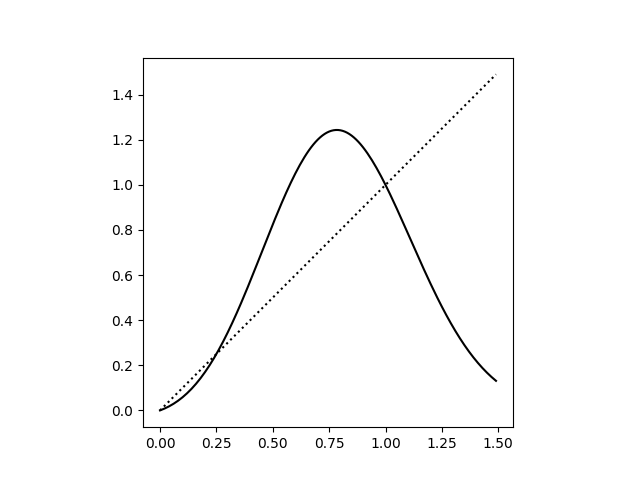
\includegraphics[width=0.5\textwidth]{figures/fig1a.png}
  \caption{Example growth function satisfying our hypotheses.}
\end{figure}

% The main result is that, starting with step initial data, two distinct outcomes are possible depending on the specific shape of the growth curve:
% \begin{enumerate}
%   \item a stacked wave train consisting of a monostable traveling wave connecting $u=0$ to $u=1$ and a 2-periodic traveling wave connecting $u=1$ to the 2-cycle $u=u^\pm$;
%   \item a bistable 2-periodic traveling wave connecting $u=0$ to $u=u^\pm$.
% \end{enumerate}

% \subsection{Integrodifference equations}
% An integrodifference equation is an integral recurrence relation on a function space in the form
% \begin{equation} \label{eqn:ide}
% u_{t+1}(x) = Q[u_t](x) = \int_{-\infty}^{\infty} k(x-y) f(u_t(y)) dy
% \end{equation}
% where $k:\mathbb{R}\to[0,\infty)$ is a probability density function called the dispersal kernel, $f:[0,\infty)\to[0,\infty)$ is called the growth function, and each $u_t:\mathbb{R}\to [0,\infty)$ is continuous.


% \subsection{Strong Allee effect and overcompensation}


% We investigated traveling wave fronts in integrodifference equations (IDEs) with growth functions exhibiting both a strong Allee effect and a stable periodic cycle. We chose a growth function $f: [0,\infty)\to[0,\infty)$ such that there exist constants $0<a<u^-<1<u^+$ such that

% \begin{enumerate}

% \item $f(0)=0$, $f(a)=a$, and $f(1)=1$,

% \item $f(u^+)=u^-$, $f(u^-)=u^+$, $f^2(u^+)=u^+$, and $f^2(u^-)=u^-$

% \item $0$ is a stable fixed point

% \item $a$ and $1$ are unstable fixed points

% \item $u^+$ and $u^-$ form a stable 2-cycle.

% \end{enumerate}

% \begin{figure}
%      \centering
%      \includegraphics[width=0.5\textwidth]{growth.png}
%      \caption{Example growth function satisfying our hypotheses.}
% \end{figure}

\subsection{Traveling waves}

A solution $(u_t)_{t=0}^{\infty}$ to equation \eqref{eqn:ide} is called a traveling wave (or traveling front) if there exists $w \in C(\mathbb{R},[0,\infty))$ and $c \in \mathbb{R}$ called the wave speed (or wave velocity) such that
\begin{equation} \label{eqn:tw1}
u_t(x) = w(x-tc)
\end{equation}
for all $t$ and $x$. Additionally we assume $w$ has limits at $\pm\infty$, which are necessarily fixed points of $f$. Equivalently, a traveling wave is a solution to the equation
\begin{equation} \label{eqn:tw2}
Q[w](x) = w(x-c)
\end{equation}
for some $c$. More generally, a $p$-periodic traveling wave is a solution to the equation
\begin{equation} \label{eqn:ptw}
Q^p[w](x) = w(x-pc)
\end{equation}
for some $c$ such that $w$ has limits at $\pm\infty$ (which are necessarily $p$-periodic points of $f$).
A periodic traveling wave is called bistable if both $w(+\infty)$ and $w(-\infty)$ belong to a stable cycle of $f$, and monostable if only one belongs to a stable cycle.

\subsection{Stacked waves and dynamical stabilization}

A stacked wave refers to a solution of \eqref{eqn:ide} which consists of multiple superimposed traveling waves with distinct velocities that disperse as $t \to \infty$; see Figure \ref{fig:ricker_waves}.
Such solutions were observed in \cite{kot1992} and rigorously analyzed in \cite{bourgeois2020}.
They were shown to occur for the logistic growth function
\begin{equation} \label{eqn:logistic}
f(u)=ru(1-u)
\end{equation}
and the Ricker growth function
\begin{equation} \label{eqn:ricker}
f(u)=u\exp(r(1-u))
\end{equation}
which both exhibit period-doubling cascades as the growth parameter $r$ increases.
A necessary (but not sufficient) condition for the existence of a stacked wave solution is a pair of traveling waves $w_1$ and $w_2$ with corresponding wave speeds $c_1$ and $c_2$ such that $w_1(+\infty) = w_2(-\infty)$ and $c_1 < c_2$.

For instance, \cite{kot1992} considered the logistic growth function with a stable 2-cycle paired with the Laplace kernel, and initial data of the form \eqref{eqn:initial_data}. The solution was shown numerically to quickly converge to a pair of stacked waves $w_1$ and $w_2$ with $w_1(-\infty)=0$, $w_1(+\infty)=w_2(-\infty)=1$ and $w_2(+\infty)=u^+$. This phenomenon has been referred to as "dynamical stabilization" because we have
$$
u_t(x) \approx 1, \quad \forall x \in [c_1t,c_2t]
$$
so that the solution attains the value of an unstable fixed point ($u=1$) on an interval which grows in length as $t \to \infty$.

\begin{figure}
  \centering
  \begin{subfigure}[b]{0.45\textwidth}
      \centering
      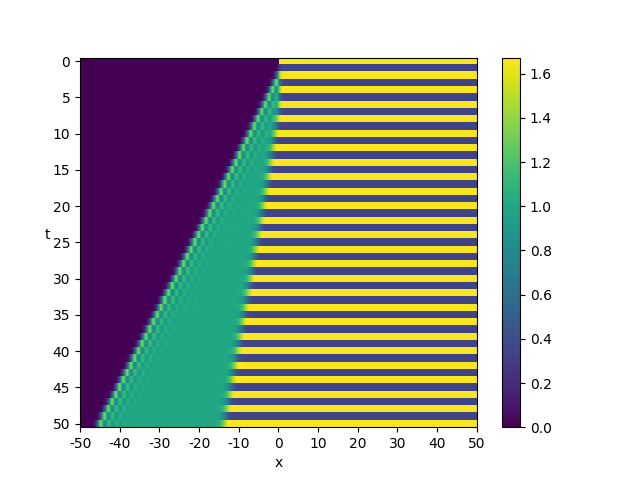
\includegraphics[width=\textwidth]{figures/fig2a.png}
      \caption{}
  \end{subfigure}
  \hfill
  \begin{subfigure}[b]{0.45\textwidth}
      \centering
      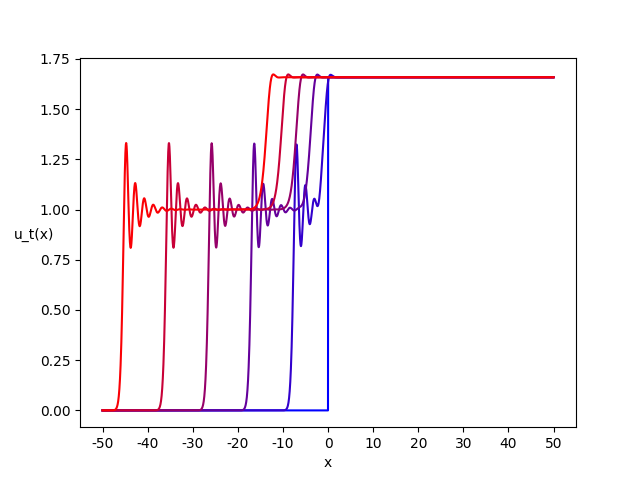
\includegraphics[width=\textwidth]{figures/fig2b.png}
      \caption{}
  \end{subfigure}
     \begin{subfigure}[b]{0.45\textwidth}
      \centering
      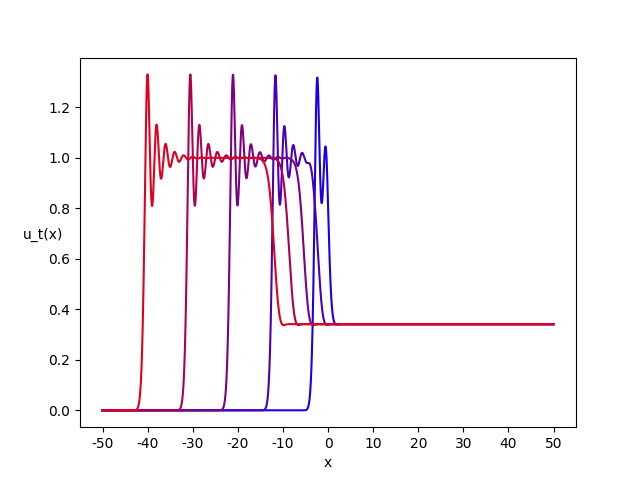
\includegraphics[width=\textwidth]{figures/fig2c.png}
      \caption{}
  \end{subfigure}
  \caption{Convergence to stacked traveling waves using the Ricker function \eqref{eqn:ricker} with $r=2.4$, Laplace dispersal kernel, and initial data $u_0(x) = u^+H(x)$. (a) shows the space-time heatmap of the solution. (b) shows the solution curves on time steps $t=0,10,20,...$ while (c) shows the solution curves on $t=5,15,25,...$, and the color changes from blue to red as $t$ increases.}
  \label{fig:ricker_waves}
\end{figure}

\section{Model and simulations}

We used the following 2-parameter growth function
\begin{equation} \label{eqn:modified_ricker}
f(u) = u \exp \left( r (1 - u) ( u - a ) \right)
\end{equation}
where $r \geq 0$ and $0 < a < 1$.
This map is a reparameterization of the growth map used in \cite{otto2022},
\begin{equation} \label{eqn:modified_ricker}
f(u) = u \exp \left( R (1 - u) ( \frac{u}{a} - 1 ) \right)
\end{equation}
via $R = ra$.

This map has a period-doubling cascase for each choice of $a$; that is, a sequence $(r_{a,n})_{n=0}^{\infty}$ (depending on $a$) such that, whenever $r_{a,n} < r < r_{a,(n+1)}$ then the growth map has a stable $2^n$-cycle and unstable $2^k$-cycles for $k = 0, ..., (n-1)$. Our conditions are therefore satisfied whenever
\begin{equation}
  r_{a,1} < r < r_{a,2}
\end{equation}

For ease of calculation \eqref{eqn:modified_ricker} can be expressed as
\begin{equation}
f(u) = u\exp(rp(u)); \quad p(u) = (1-u)(u-a)
\end{equation}
Its first derivative is
\begin{equation} \label{eqn:modified_ricker}
f'(u) = (1+rup'(u))\exp(rp(u)) = (1 + r(a+1)u - 2ru^2) \exp \left( r (1 - u) ( u - a ) \right)
\end{equation}
We can determine its monotonicity and the stability of the fixed points by computing
\begin{enumerate}
\item $f'(0) = \exp \left( -ar \right)  \in (0,1)$,
\item $f'(a) = 1 + ra(1-a) \in (1,\infty)$, and
\item $f'(1) = 1 - r(1-a)$.
\end{enumerate}
So, $u=0$ is always stable and $u=a$ is always unstable.  Assuming $r>0$, we have
\begin{equation}
f'(1)<0 \quad \iff \quad r < \frac{1}{1-a} \quad \implies f \text{ is monotone on } [0,1] \implies u=1 \text{ is stable}
\end{equation}
Therefore,
\begin{equation} \label{eqn:modified_ricker}
u=1 \text{ is stable} \quad \Leftarrow \quad |f'(1)|<1 \quad \iff \quad r < \frac{2}{1-a}
\end{equation}
We have,
\begin{equation}
  r_{a,0}=0; \quad r_{a,1}=\frac{2}{1-a}
\end{equation}
Computing $r_{a,2}$ is not straightforward and involves solving a transcendental equation $f^2(u)=u$ where $f^2 = f \circ f$ is the second-iterate map,
\begin{equation} \label{eqn:modified_ricker}
\begin{aligned}
f^2(u) &= f(u) \exp \left( r p(f(u)) \right) \\
&= u \exp \left( r (1 - u) ( u - a ) + r (1 - u \exp \left( r (1 - u) ( u - a ) \right)) ( u \exp \left( r (1 - u) ( u - a ) \right) - a ) \right)
\end{aligned}
\end{equation}
Locating the 2-periodic points thus amounts to solving the equation
\begin{equation}
f^2(u) = u \quad \iff \quad p(u) + p(u\exp(rp(u))) = 0
\end{equation}

In practice, assuming $r_{a,1} < r<r_{a,2}$, a numerical scheme can be used to estimate $u^\pm$ by perturbing the unstable fixed point.

%\begin{equation}
%u^+ \approx \max ( f^n(1+\epsilon), f^{n+1}(1+\epsilon)); \quad 0 < \epsilon \ll 1; \quad  n \gg 0
%\end{equation}

The initial data is given by the step function
\begin{equation} \label{eqn:initial_data}
u_0(x) = \begin{cases}
0 & x < 0 \\
u^+ & x \geq 0
\end{cases}
\end{equation}



% Furthermore, there is an increasing sequence $r_{1,a},r_{2,a},r_{3,a},...$ (depending on $a$) of period-doubling bifurcation points such that
% \begin{itemize}
% \item if $0<r<r_{1,a}$ then $u=1$ is a stable fixed point
% \item if $r_{1,a}<r<r_{2,a}$ then $u=1$ is an unstable fixed point and there is a stable 2-cycle.
% \item if $r_{2,a}<r<r_{3,a}$ then $u=1$ is unstable, there is an unstable 2-cycle, and a stable 4-cycle,
% \item in general, if $r_{n,a}<r<r_{(n+1),a}$, there are unstable $2^k$-cycles for each $k=0,1,...,(n-1)$, and a stable $2^n$-cycle.
% \end{itemize}
% Thus, we focus on the case when $r \in (r_{1,a},r_{2,a})$.
% For the dispersal kernel, we used either the Gaussian kernel, Laplace kernel, or uniform kernel.
% We use step initial data in the form \eqref{eqn:initial_data}.

%\subsection{Two stacked waves or one bistable wave}

The model with initial condition \eqref{eqn:initial_data} exhibits two distinct behaviors, depending on the model parameters, as illustrated below in Figure \ref{fig:modified_ricker_waves}. Either:
\begin{enumerate}[Outcome 1.]
  \item a single bistable 2-periodic traveling wave connecting $u=0$ to $u=u^\pm$ (as shown in the left column of Figure \ref{fig:modified_ricker_waves});
  \item a pair of monostable traveling waves that form a stacked wave train, connecting $u=0$ to $u=1$ and $u=1$ to $u=u^\pm$, respectively (as shown in the right column of Figure \ref{fig:modified_ricker_waves}).
\end{enumerate}
This observation naturally leads to several questions:
\begin{enumerate}[Q1.]
  \item for what regions of the parameter space does dynamical stability/a stacked traveling front occur, vs a periodic traveling wave?
  \item can we prove existence/stability of the wave in either case?
  \item is there a general formula, as in \cite{wang2002}, that could guarantee/forbid the existence of this wave? For example, if there is a wave $w_1$ with $w_1(-\infty)=0$ and $w_1(+\infty)=1$ and a periodic traveling wave $w_2$ with $w_2(-\infty)=1$ and $w_2(+\infty)=u^+$, with speeds $c_1$ and $c_2$ respectively, is $c_1>c_2$ a necessary/sufficient condition?
\end{enumerate}

\begin{figure}
     \centering
     \begin{subfigure}[b]{0.45\textwidth}
      \centering
      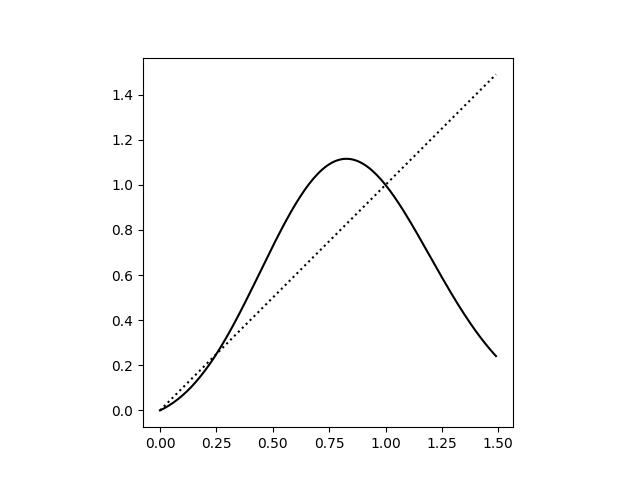
\includegraphics[width=\textwidth]{figures/fig3_growth1.png}
      \caption{}
  \end{subfigure}
  \begin{subfigure}[b]{0.45\textwidth}
      \centering
      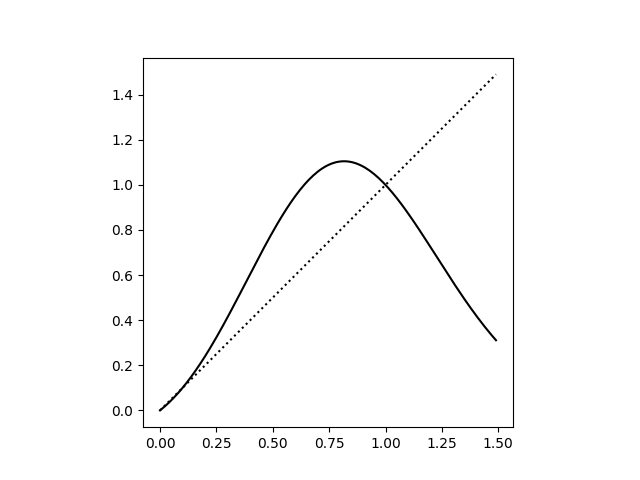
\includegraphics[width=\textwidth]{figures/fig3_growth2.png}
      \caption{}
  \end{subfigure}
     \begin{subfigure}[b]{0.45\textwidth}
         \centering
         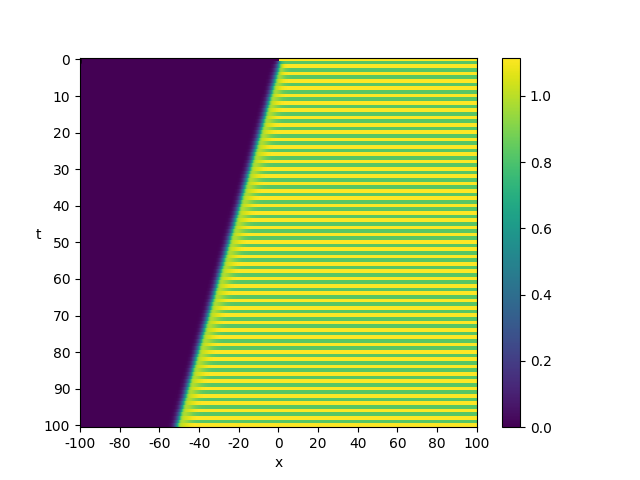
\includegraphics[width=\textwidth]{figures/fig3a.png}
         \caption{}
     \end{subfigure}
     \begin{subfigure}[b]{0.45\textwidth}
         \centering
         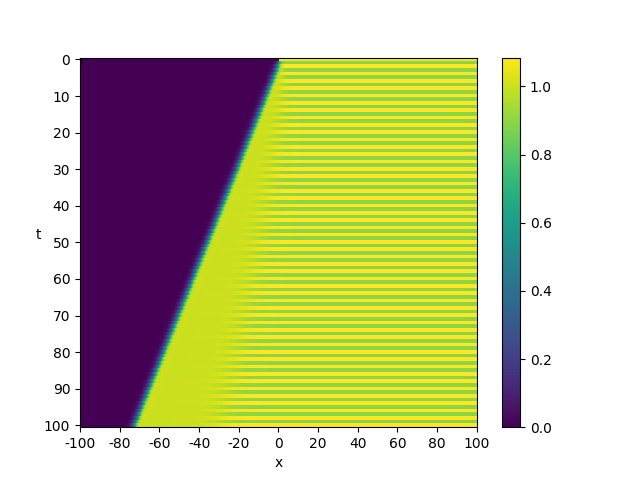
\includegraphics[width=\textwidth]{figures/fig3d.png}
         \caption{}
     \end{subfigure}
     \begin{subfigure}[b]{0.45\textwidth}
      \centering
      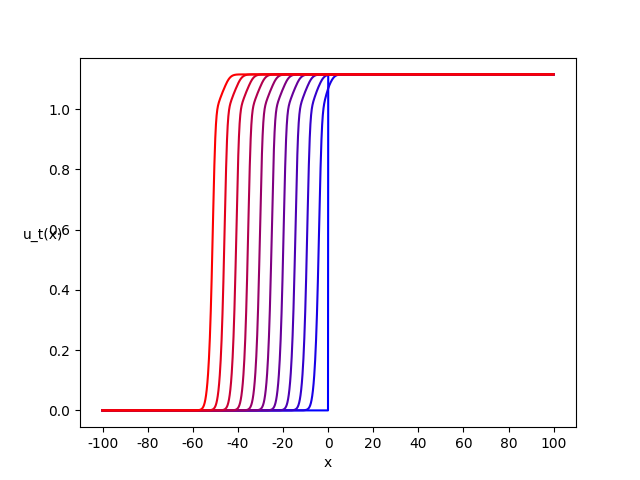
\includegraphics[width=\textwidth]{figures/fig3b.png}
      \caption{}
  \end{subfigure}
  \begin{subfigure}[b]{0.45\textwidth}
    \centering
    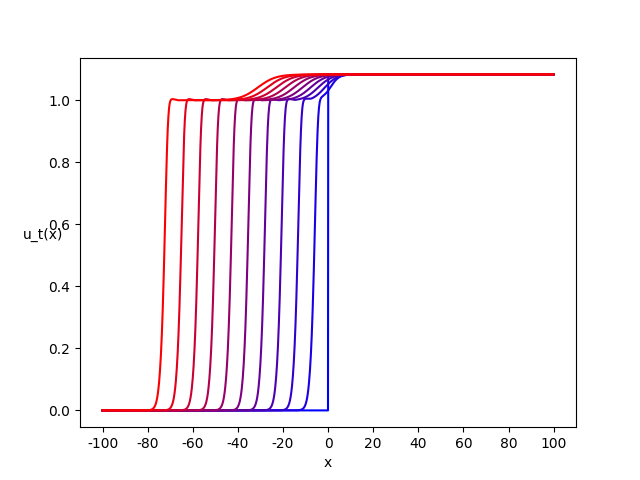
\includegraphics[width=\textwidth]{figures/fig3e.png}
    \caption{}
\end{subfigure}
\begin{subfigure}[b]{0.45\textwidth}
  \centering
  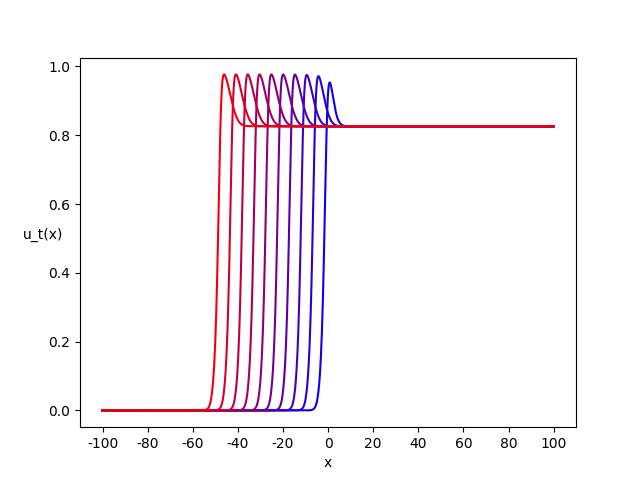
\includegraphics[width=\textwidth]{figures/fig3c.png}
  \caption{}
\end{subfigure}
\begin{subfigure}[b]{0.45\textwidth}
  \centering
  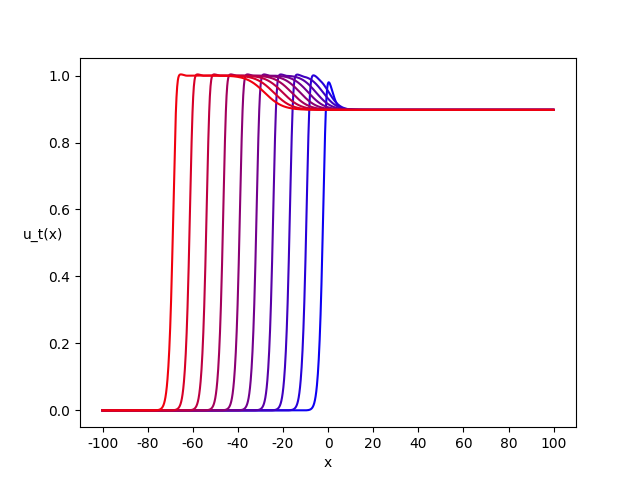
\includegraphics[width=\textwidth]{figures/fig3f.png}
  \caption{}
\end{subfigure}
        \caption{The left and right columns show our growth function \eqref{eqn:modified_ricker} with parameters $(a=0.25, r=3.0)$ and $(a=0.1,r=2.3)$ respectively. (a) and (b) show the plot of the growth curve, while (c) and (d) show convergence to a pair of stacked waves vs. a single 2-periodic traveling wave, respecively.}
        \label{fig:modified_ricker_waves}
\end{figure}

\printbibliography
\end{document}